\chapter{Background}\label{chap:bkg}

%TODO more math and explain it

\section{Cell-free systems}
\gls{cfps} systems have existed since the early 1960's as a way to express proteins that are otherwise difficult to express in a living cell~\cite{nirenberg1961dependence}.
These early \gls{cfps} systems were quite crude and had low protein yields, limiting their utility.
More recently, work involving the removal of certain genes~\cite{calhoun2006total} and the improved stability of cofactor regeneration pathways~\cite{jewett2008integrated}, has improved the yield of \gls{cfps} systems.
%stabilized amino acid synthesis leading to 
%Another crucial development was the ability to ensure cofactor regeneration pathways were maintained in the \gls{cfps} system}.
%These recent improvements in \gls{cfps} systems have led to a multitude of applications for cell-free technologies~\cite{}.

When discussing \gls{cfps} systems, it is important to distinguish between the multiple types of cell-free systems.
One type of cell-free system is created by combining individual purified proteins involved in transcription and translation.
The most widely utilized of these reconstituted cell-free systems is the PURE system~\cite{shimizu2001cell}.
The benefit of these systems is that the system is completely known and controlled.
Since the only things in the system are the proteins that have been deliberately added, users of the systems can be assured that there are no undesirable elements such as nucleases or proteases present.
However, these systems have relatively high costs due to the time and effort required to isolate and purify each of the requisite proteins.

The type of \gls{cfps} system we use in this dissertation is an extract-based system created using a crude cell extract.
Creating an extract-based \gls{cfps} system involves growing cells and then lysing them to create a cell extract.
This extract is then used as the basis of the \gls{cfps} system with the assumption that all the important transcription/translation machinery remains intact in the cell extract.
These systems are also known as \gls{tx}/\gls{tl} systems for this reason.
Growing large quantities of cells is relatively cheap, so these types of systems have the potential to scale more effectively than reconstituted cell-free systems. 
The downside to this method of creating \gls{cfps} systems is that the exact composition of these cell extracts is unknown and can potentially vary between batches of \gls{cfps} systems.
This motivates our work to provide an accurate model of these crude \gls{cfps} systems.

\section{Flux Balance Analysis}
Flux Balance Analysis (\gls{fba}) is one of the most common metabolic modeling tools.
\gls{fba} relies on a mathematical representation of all of the metabolic reactions occurring in an organism.
These reactions are represented using a matrix $S$, a $M \times N$ matrix, where each row represents a separate reaction and each column is a different metabolite.
The entries in this matrix are the stoichiometric coefficient for each metabolite in a given reaction.
Metabolites that are consumed in a reaction are represented using negative numbers.
Flux through each of these reactions can be represented by a vector $v$, which is a 1-dimension vector with a length equal to the number of the reactions.
A crucial assumption in \gls{fba} is that the system is at steady state, so the overall flux through all of the reactions is not changing.
We can represent this by writing the following:
\begin{equation}
S \times v = \vec{0} \\
\end{equation}
where $S$ is the known stoichiometric matrix and $v$ is the unknown flux vector.
The goal of \gls{fba} is to solve for $v$.

This system is underspecified---there are typically more reactions than metabolites ($N >> M$)---so there is no unique solution to this equation.
This issue is solved by specifying a specific objective function to optimize for as well as adding constraints to our flux vector $v$.
We can specify constraints on different reactions in order to limit the amount of flux proceeding through a given reaction.
For instance, we represent a reaction as irreversible by setting the lower bound on that reaction to be 0.
This specifies that it can only proceed in one direction and ensures that the model reflects the underlying biology.
We use \gls{lp} to solve this constrained, underspecified system. 

In order to find an optimal solution to this problem, we first need to specify an objective function.
This objective function determines which fluxes are most phenotypically relevant.
When choosing an objective function, we can either choose a specific reaction in which to optimize the flux or create a pseudo-reaction that contains a combination of important metabolites.
A common choice of objective function is the Biomass Objective Function, which incorporates many essential metabolites necessary for cell growth~\cite{feist2010biomass}.
While some of our models use the Biomass Objective Function, we also use the production of a specific product as our objective function.
In the general case, we can represent our objective function as $Z$.
%TODO clean up
We specify which reactions are part of the objective function using the vector $c$.
When the objective function is just the optimization of a single reaction (e.g. production of a desired product), $c$ is extremely sparse, having only a single entry.
However, $c$ can also have multiple entries when the objective function is a linear combination of desired products.

Now we can reformulate our problem to be a \gls{lp} problem of the form:
\begin{equation}
\centering
\begin{split}
\text{max } Z &= c^Tv \\
&\text{s.t. } S \times v = \vec{0} \\
&\text{and } -\inf < v_0 < \inf \\
&\text{and } 0 < v_1 < \inf \\
&\text{and } 0 < v_2 < 10 \\
...
\end{split}
\end{equation}
where $v_i$ is the flux through reaction $i$.
$v_0$ is an example of a reversible reaction because flux can go either way.
$v_1$ is irreversible, but unconstrained, while $v_2$ is irreversible but constrained due to some limiting factor.
We can then use a \gls{lp} solver to find the optimal solution to this problem.
%It may be useful to imagine the potential space of all \gls{fba} solutions that can satisfy the constraints as a hypercube.
%Then, the linear programming solver finds an optimum at one corner of the hypercube based on the objective function.

The use of \gls{fba} involves this key steady state assumption---i.e. the system is stable.
\gls{cfps} systems are dynamic systems and do not have a period where intake and output are equal until the system is no longer producing protein.
However, we can consider the period of maximal production of a \gls{cfps} system to be its steady state.
Thus, we can use \gls{fba} to analyze this pseudo-steady state, which is the interval that we are interested in.

%A typical \gls{fba} model includes thousands of reactions; this is extremely high dimensional data.
%In order to extract insights from the data, we need to use dimensionality reduction techniques.

\section{Autoencoders}
Autoencoders are a dimensionality reduction technique with a simple idea: given a dataset, try to reconstruct that dataset by passing it through a lower dimensional subspace.
Deep autoencoders, which we will just refer to as autoencoders, use two neural networks to accomplish this.
One network, which we will refer to as an encoder, performs the mapping from the original dataset to the lower dimensional subspace.
A second network, called the decoder, attempts to reconstruct the original dataset by mapping back from the lower dimension back to the dimension of the original dataset.
The original idea behind autoencoders was that this lower dimensional representation of the data served as a compressed version of the data.
Instead of hand designing compression/decompression algorithms, these functions can be learned by a neural network and can therefore be application specific.
In practice, these autoencoders often perform worse than hand-designed compression algorithms.
For instance, autoencoders have difficulty competing with classic algorithms on well-studied problems such as image compression~\cite{theis2017lossy}.
However, autoencoders can also be used as a dimensionality reduction technique.

The lower dimensional subspace that the autoencoders map has been shown to be an effective form of unsupervised dimensionality reduction~\cite{baldi2012autoencoders}.
The transformations that autoencoders learn can sometimes uncover hidden relationships in the data that may be non-obvious in the original dataset.
Biologists often use \gls{pca} to achieve similar goals.
\gls{pca} also projects the data into a subspace, but it does so in a linear manner.
Autoencoders have the advantage that they are able to learn non-linear transformations.

\begin{figure}[t!]
\begin{center}
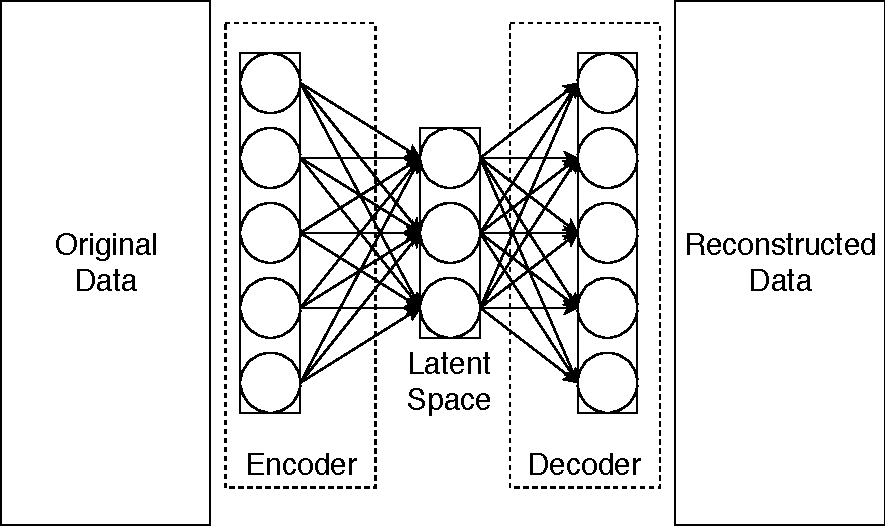
\includegraphics{figs/Autoencoder.pdf}
\caption[Example of a single layer autoencoder]{Example of a single layer autoencoder.
In this case, both the encoder and the decoder are a single layer neural network.
These layers can be stacked to create even more complex dimensionality reductions.}
\end{center}
\label{fig:ae}
\end{figure}

Figure \ref{fig:ae} demonstrates the structure of a very simple autoencoder.
While the main idea of an autoencoder is unchanged, there are a number of different version of autoencoders that are extensions of this basic idea.
One example is a sparse autoencoder.
In order to force the autoencoder to learn a more general dimensionality reduction, we can add a sparsity constraint to limit the number of activations among the network layers.
This forces the autoencoder to learn a representation with sparse network weights.
Another type of autoencoder is a denoising autoencoder.
This type of autoencoder involves taking a noisy representation and mapping it to a clean representation of the data.
These autoencoders add noise to the original data and then try to learn the original representation from the corrupted data.
Despite their differences, almost all of these autoencoder types are trained using reconstruction loss---a measure of how far the autoencoded data is from the original data.

Sometimes we want to do more than just learn arbitrary encoding and decoding functions.
For instance, we might want to impose constraints on the encoded representation.
\glspl{vae} are a class of autoencoder that does exactly this.
\glspl{vae} constrain the encoded representation to be a probability distribution.
So, instead of learning deterministic functions to encode/decode the data, a \gls{vae} learns a mapping to parameters of an encoded probability distribution.
Throughout this work, we will use a normal distribution as our encoded distribution, though other distributions can also be used with \glspl{vae}.
Thus, the encoder learns to map samples to the mean and standard deviation of the normal distribution.
Borrowing terminology from the field of probabilistic models, we call this our latent space.
In order to decode a data point, we can sample from the encoded probability distribution to generate a reconstruction in the original dimension.

\glspl{vae} measure loss using a combination of two loss terms.
Firstly, we care about how well we are able to reconstruct our original data.
So, we keep a reconstruction loss term to measure how well the reconstructed data mimics the original data.
Our second loss term acts as a regularizer on the latent space and constrains it to be well formed.
This term is calculated using \gls{kl} divergence, a common way of measuring difference between probability distributions.
We can compute the the \gls{kl} divergence between our latent space and a prior distribution, which in most cases is a normal distribution.
With the combination of those two loss terms, we can then train the \gls{vae} as we would any other neural network---by using gradient descent to minimize the loss function.

Let $x_i \in X$ be our data and $z$ the latent representation learned by the \gls{vae}.
Our encoder network can be represented by the function $p$ which has parameters $\theta$.
Similarly, our decoder can be represented as a posterior distribution $q$ that is parameterized by $\phi$.
Then the loss function of a \gls{vae} can therefore be written out as follows:

\begin{equation}\label{eqn:vae-loss}
\mathcal{L}(\theta, \phi) = - E[\log p_{\theta}(x_i | z)] + KL(q_{\phi}(z | x_i) || p(z)) \\
\end{equation}

Minimizing this first part of the loss involves reducing the reconstruction error by maximizing the probability of reconstructing the original data given our latent representation.
Minimizing the second part of the loss requires the latent representation to be similar to our prior distribution.
We learn the $\theta$ and $\phi$ terms that minimizes this function.
%TODO: add here